%! TEX Program = pdflatex

\documentclass{article}
\usepackage[a4paper,margin=1cm,left=2cm,right=2cm]{geometry}
\usepackage{newtxtext}
\usepackage{graphicx}
\usepackage{url}
\usepackage[colorlinks, urlcolor=blue]{hyperref}
\title{\huge Hall Effect --- Helmholtz Coil}
\author{Teddy van Jerry}
\date{\today}
\pagenumbering{gobble}
\renewcommand{\ttdefault}{pcr}

\begin{document}
    \maketitle

    Figures below are drawn using \texttt{MATLAB 2021a}.
    The \texttt{MATLAB} code is open source on GitHub under the MIT License: \url{https://github.com/Teddy-van-Jerry/SEU_Physics_Experiment}, \texttt{Hall Effect}.

    It has helped some of my classmates in drawing an elegant figure.

    \begin{figure}[htbp]
        \centering
        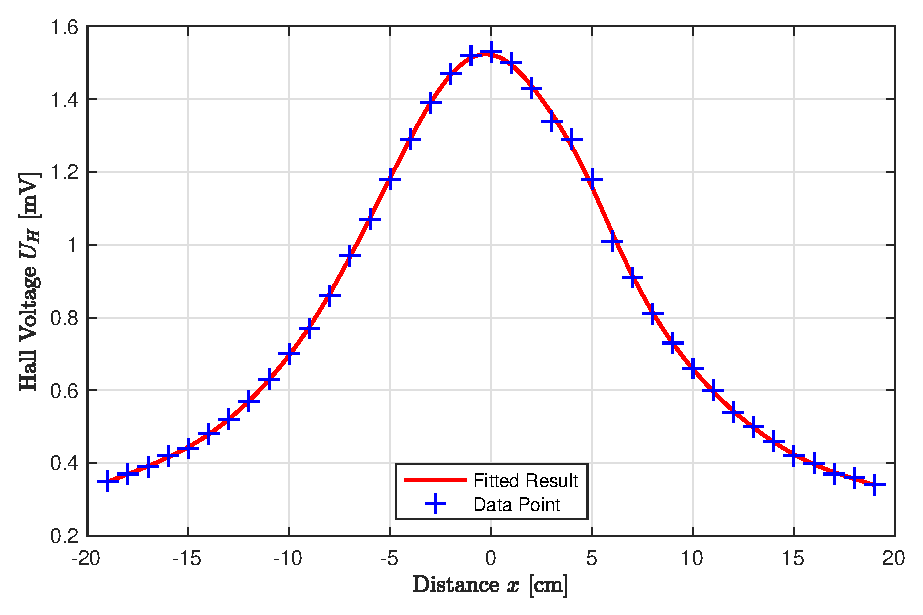
\includegraphics[width=.75\linewidth]{One.eps}
        \caption{$U_H$ vs. $x$ with one coil}
        \label{fig:one}
    \end{figure}
    \begin{figure}[htbp]
        \centering
        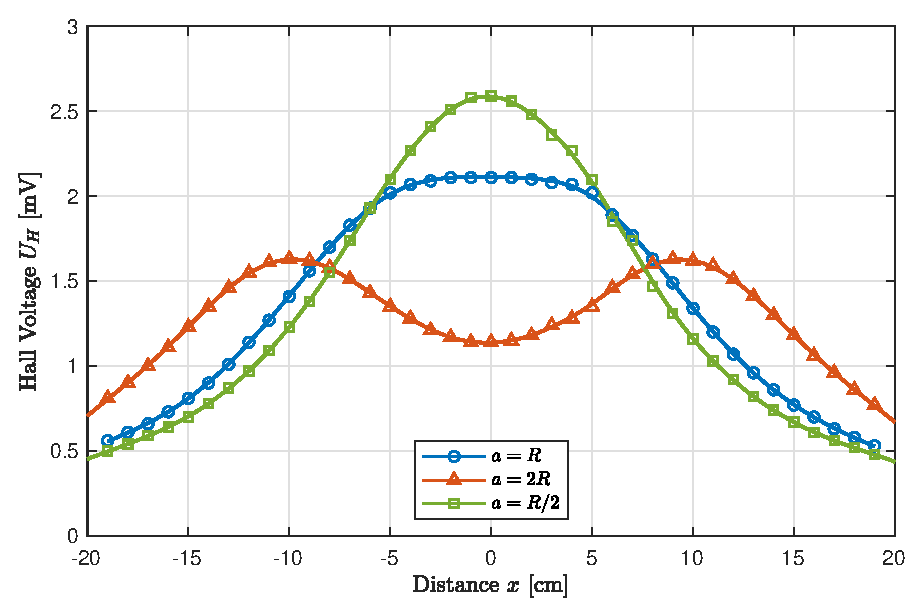
\includegraphics[width=.75\linewidth]{Two.eps}
        \caption{$U_H$ vs. $x$ with two coils}
        \label{fig:two}
    \end{figure}
\end{document}

% ALL RIGHTS RESERVED (C) Teddy van Jerry
